\begin{frame}[fragile]
\frametitle{How to Diagnose Load Imbalance}
\begin{itemize}
 \item Often hidden in statements such as:
 \begin{itemize}
  \item Very high synchronization overhead
  \begin{itemize}
   \item Most processors are waiting at a reduction
  \end{itemize}
 \end{itemize}
 \item Count total amount of computation (ops/flops) per processor
 \begin{itemize}
  \item In each phase! 
  \item Because the balance may change from phase to phase
 \end{itemize}
\end{itemize}
\end{frame}

\begin{frame}[fragile]
\frametitle{Golden Rule of Load Balancing}
\emph{Fallacy: objective of load balancing is to minimize variance in load across processors}

\begin{itemize}
 \item[]\emph{Example:}
 \begin{itemize}
  \item  50,000 tasks of equal size, 500  processors:
  \begin{itemize}
   \item A: All processors get 99, except last 5 gets $100+99 = 199$
   \item OR, B:  All processors have 101, except last 5 get 1
  \end{itemize}
 \end{itemize}
 \item[] Identical variance, but situation A is much worse!
\end{itemize}


\emph{Golden Rule: It is ok if a few processors idle, but avoid having processors that are overloaded with work}


\emph{Finish time} = maxi(Time on processor i)
\begin{itemize}
\item[] excepting data dependence and communication overhead issues
\end{itemize}

The speed of any group is the speed of slowest member of that group.
\end{frame}

\begin{frame}[fragile]
\frametitle{Grainsize and Load Balancing}
\begin{itemize}
\item[] How Much Balance Is Possible?
\end{itemize}
\begin{centering}
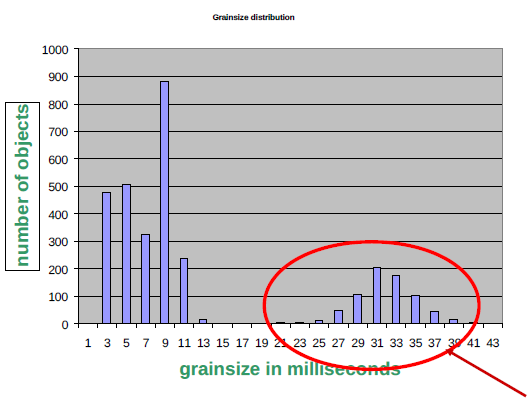
\includegraphics[width=0.8\textwidth]{figures/histogramGrains}
\end{centering}
\end{frame}

\begin{frame}[fragile]
\frametitle{Automatic Dynamic Load Balancing}
\begin{itemize}
\item Measurement based load balancers
\begin{itemize}
\item Principle of persistence: In many CSE applications, computational loads and communication patterns tend to persist, even in dynamic computations
\item Therefore, recent past is a good predictor of near future
\item Charm++ provides a suite of load-balancers 
\item Periodic measurement and migration of objects
\end{itemize}
\item Seed balancers (for task-parallelism)
\begin{itemize}
\item Useful for divide-and-conquer and state-space-search applications
\item Seeds for charm++ objects moved around until they take root
\end{itemize}
\end{itemize}
\end{frame}

\begin{frame}[fragile]
\frametitle{Using the Load Balancer}
\begin{itemize}
\item link a LB module 
\begin{itemize}
\item \code{-module <strategy>}
\item RefineLB, NeighborLB, GreedyCommLB, others…
\item EveryLB will include all load balancing strategies
\end{itemize}
\item compile time option (specify default balancer)
\begin{itemize}
\item \code{-balancer RefineLB}
\item runtime option
\item \code {+balancer RefineLB}
\end{itemize}
\end{itemize}
\end{frame}

\begin{frame}
\frametitle{Code to Use Load Balancing}
\begin{itemize}
\item Insert \code{if (myLBStep) AtSync() else ResumeFromSync();} call at natural barrier
\item Implement \code{ResumeFromSync()} to resume execution
\begin{itemize}
\item Typical ResumeFromSync contribute to a reduction
\end{itemize}
\end{itemize}
\end{frame}

\begin{frame}[fragile]
\frametitle{Example: Stencil}
\begin{lstlisting}[basicstyle=\tiny]
while (!converged) {
  atomic {
    int x = thisIndex.x, y = thisIndex.y, z = thisIndex.z;
    copyToBoundaries();
    thisProxy(wrapX(x-1),y,z).updateGhosts(i, RIGHT, dimY, dimZ, right);
    /* ...similar calls to send the 6 boundaries... */
    thisProxy(x,y,wrapZ(z+1)).updateGhosts(i, FRONT, dimX, dimY, front);
  }
  for (remoteCount = 0; remoteCount < 6; remoteCount++) {
    when updateGhosts[i](int i, int d, int w, int h, double b[w*h])
    atomic { updateBoundary(d, w, h, b); }
  }
  atomic {
    int c = computeKernel() < DELTA;
    CkCallback cb(CkReductionTarget(Jacobi, checkConverged), thisProxy);
    if (i%5 == 1) contribute(sizeof(int), \&c, CkReduction::logical_and, cb);
  }
  if (i % lbPeriod == 0) { atomic { AtSync(); } when ResumeFromSync() {} }
  if (++i % 5 == 0) {
    when checkConverged(bool result) atomic {
      if (result) { mainProxy.done(); converged = true; }
    }
  }
}
\end{lstlisting}
\end{frame}

\begin{frame}
\frametitle{Performance}
\begin{centering}
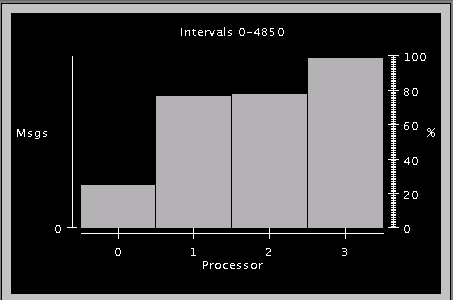
\includegraphics[width=0.5\textwidth]{figures/beforeLB}
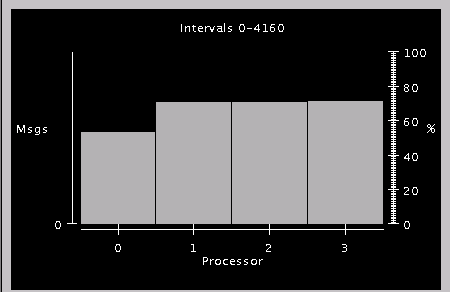
\includegraphics[width=0.5\textwidth]{figures/afterLB}
\end{centering}
\end{frame}
